Here first the limitations of Scikit-learn predefined ML models - Logistic Regression(LR) and Multi-Layer-Perceptron(MLP), are described. The Logistic Regression Model seems to work almost perfectly with all 3 classes when the bad region size is $5\times5$ (as in \autoref{Occupancymaps5x5}) with either the same or randomized location. When the bad region size is 1x1 like in \autoref{Ocuppancymaps1x1} the LR Model performs poorly with an accuracy of approximately 20\%.
 The MLP does not seem to work in any of the used cases that are studied as it always performs poorly with an accuracy of $\approx 40\%$.

\begin{figure}[h]
\centering
\begin{subfigure}[t]{.316\textwidth}
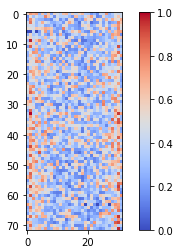
\includegraphics[width=\textwidth]{Good_image_1x1.png}
\caption{}
\end{subfigure}
\begin{subfigure}[t]{.305\textwidth}
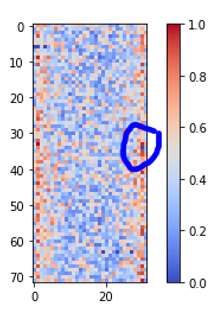
\includegraphics[width=\textwidth]{Dead_image_1x1.png}
\caption{}
\end{subfigure}
\begin{subfigure}[t]{.3\textwidth}
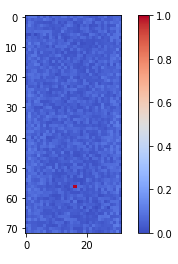
\includegraphics[width=\textwidth]{Hot_image_1x1.png}
\caption{}
\end{subfigure}
\vspace{5mm}
\caption{Occupancy Maps with 1x1 bad regions. A) Good image B) Dead image C) Hot image\label{Ocuppancymaps1x1}}
\end{figure}

Also, the use of Scikit-learn’s library is limited in comparison with the Keras module since one cannot customize the structure of the ML model with detail. Moreover, Keras is an ML library designed for developing deep neural networks. Hence it was decided to use Keras primarily for the creation of the model.
 With the Keras library, numerous models were designed with both, SL method and SSL learning method. Using SL method, we are interested in detecting anomalies and classifying what type of anomaly is seen. With SSL method, we are interested in looking at the error of the reconstruction of an image to give an idea that the image given can be considered good or that it might have some unseen anomalies

\section{SL Models for known anomalies in the HCAL data for DQM}
We considered three SL Models for classification of known anomalies in the HCAL data for DQM. 
These models are based on Convolutional Neural Networks and differ in the number of layers utilized, their ordering and number of units in each layer. The Models and the corresponding results are described below.


\subsection{Two Convolutional Layers for binary classification\label{sect:2convlayermodel}}
Several variations of the two Convolutional Layers Model were tested and optimized on the DQM data. This led to an optimal value of 8 units/neurons in the Convolutional layers. 
The detail of selecting the number of units per layer is of great importance to find a balance between efficiency and complexity of a model. More complex models (more layers and connections) are “heavy” to train in terms of computational cost, provide better results and are prone to “overfitting” to the training data.
 Simpler models (fewer layers and connections) are quicker to train, efficient and computationally economic. However, simpler models are more likely to “underfit” to the data. The \autoref{fig:2convlayermodel} below shows a code snippet with this model.
\autoref{fig:2convlayermodelfixedresults} below shows the learning curve for this model trained with Good and Hot images for fixed $5\times 5$ location and the corresponding Confusion Matrix.

\autoref{fig:2convlayermodelrandomresults} shows the learning curve for this model trained with Good and Hot images for fixed $5\times5$  location and the corresponding Confusion Matrix.

\begin{figure}
\begin{center}
    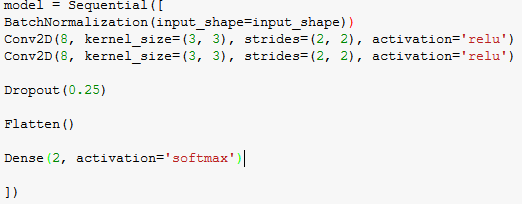
\includegraphics[width=.9\textwidth]{2_conv_layers_model.png}
\end{center}
\caption{Two Convolutional Layers Model\label{fig:2convlayermodel}}
\end{figure}


\begin{figure}
\centering
	\begin{subfigure}{.45\textwidth}
 	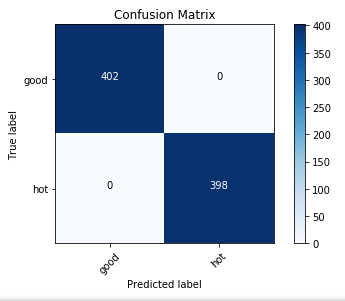
\includegraphics[width=\textwidth]{CM_2x2_with_5x5_good_hot_fixed.png}
	\end{subfigure}
	\begin{subfigure}{.45\textwidth}
	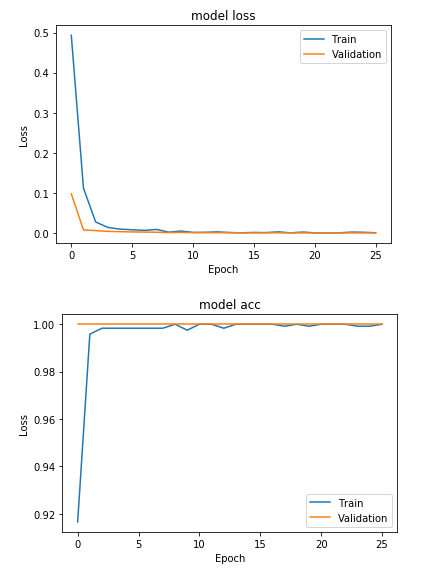
\includegraphics[width=\textwidth]{Learning_curve_5x5_good_hot_fixed.png}
	\end{subfigure}
	\caption{Confusion Matrix results and Learning curve
	 for $5\times 5$ damaged area with on the same location for all trials\label{fig:2convlayermodelfixedresults}}
 \end{figure}
 
 \begin{figure}
 	\begin{subfigure}{.45\textwidth}
 		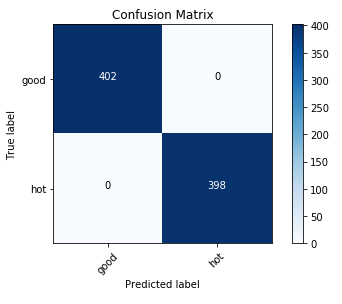
\includegraphics[width=\textwidth]{2x2CMwith_5x5_good_hot_random.png}
 	\end{subfigure}
 	\begin{subfigure}{.45\textwidth}
 	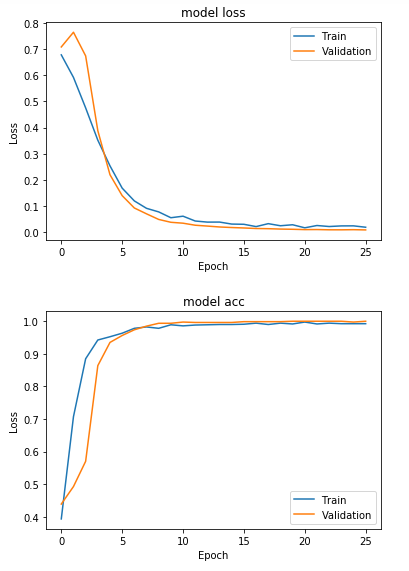
\includegraphics[width=\textwidth]{Learning_curve_5x5_good_hot_random.png}
 	\end{subfigure}
 \caption{Confusion Matrix results and Learning curve
	 for $5\times5$ damaged area with on the random location for all trials\label{fig:2convlayermodelrandomresults}}
 \end{figure}
 

\begin{figure}
	\begin{subfigure}{.5\textwidth}
 		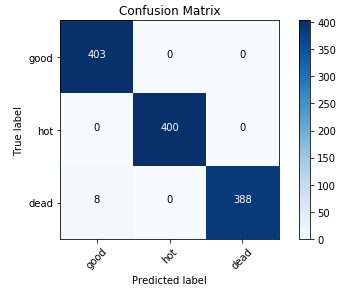
\includegraphics[width=\textwidth]{3x3CMwith_5x5_good_hot_dead_random.png}
 	\end{subfigure}
 	\begin{subfigure}{.45\textwidth}
 	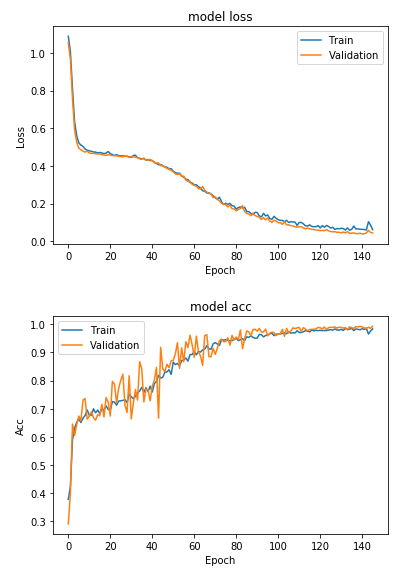
\includegraphics[width=\textwidth]{Learning_curve_5x5_good_hot_dead_random.png}
 	\end{subfigure}
 \caption{Confusion Matrix results and Learning curve
	 for $5\times5$ damaged area with an extra class to identify with random location for all trials\label{fig:2convlayermodelGHDrandomresults}}
 \end{figure}
 
\autoref{fig:2convlayermodelGHDrandomresults} shows the learning curve for this model trained with Good, Hot and Dead images for random $5\times5$ location and the corresponding Confusion Matrix

\autoref{fig:2convlayermodelGHD1x1randomresults} shows the learning curve for this model trained with Good, Hot and Dead images 
for random $1\times1 $ location and the corresponding Confusion Matrix. The corresponding learning curves and 
confusion matrix for a fixed location for 3-class (Good, Hot, Dead) configuration give the same behavior as 2-labels (Good, Hot) images



\begin{figure}
\begin{subfigure}{.5\textwidth}
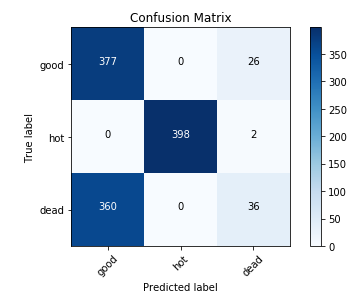
\includegraphics[width=\textwidth]{3x3CMwith_1x1_good_hot_dead_random.png}
\end{subfigure}
\begin{subfigure}{.45\textwidth}
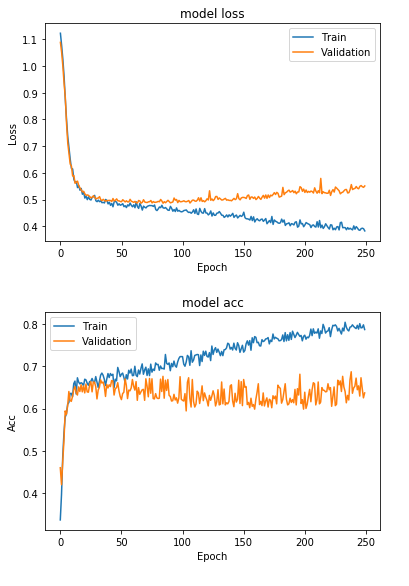
\includegraphics[width=\textwidth]{Learning_curve_1x1_good_hot_dead_random.png}
\end{subfigure}
\caption{Confusion Matrix results and Learning curve for $1\times1$ damaged area with random location for all trials
 \label{fig:2convlayermodelGHD1x1randomresults}}
\end{figure}
	
	
In a more realistic scenario, the problems with HCAL DQM would be more granular i.e. $1\times1$ type. 
When this model is tested for problematic channels in $1\times1$ configuration the learning curves for the training (\textcolor{blue}{blue}) and validation (\textcolor{orange}{orange}) sets depart after few epochs as shown in Figure 12 (right part).
From the left part of the figure, dividing the sum of numbers along the diagonal (377+398+36) by the sum of all the numbers in the matrix gives ~1/3. This demonstrates that the model is “overfitting” to the training set and misclassifies images $\approx 33\% $ of times. Hence, we consider adding a Convolutional layer to gain more prediction accuracy as shown in the next section.	
	
	
\subsection{Three Convolutional Layer for multiclass classification}
	
In this model we add another Convolutional layer to increase the prediction accuracy for a more realistic scenario in the HCAL, that is, $1\times1$ test cases and overcome the deficiency of the previous model. The code snippet in \autoref{fig:3convmodelsnippet} reflects the changes made with respect to the \autoref{sect:2convlayermodel}.



\begin{figure}
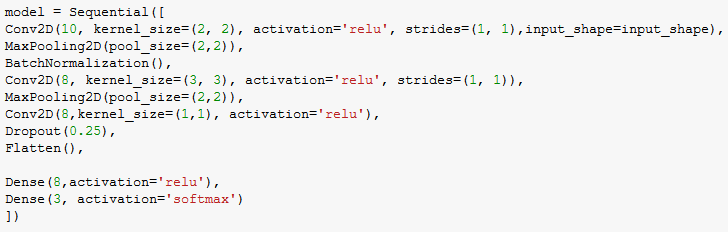
\includegraphics[width=\textwidth]{3_conv_layers_model.png}
\caption{Code snippet of a ML model with three convolutional layers for better identification\label{fig:3convmodelsnippet}}
\end{figure}
\vspace{1cm}

\autoref{fig:model2results} shows the performance of this model. The learning curves on the right-side show that the training (\textcolor{blue}{blue}) and validation (\textcolor{orange}{orange}) sets correlate well with each other. In other words, the model can successfully apply what it learns from the images. The \textbf{ROC} curve on the lower left 
shows the variation of the true positive rate (\textbf{TPR}) versus the false positive rate (\textbf{FPR}) for three classes 0, 1 and 2 corresponding to the labels Good, Hot and Dead, respectively.
 “Each point on the \textbf{ROC} curve represents a sensitivity/specificity pair corresponding to a decision threshold” \cite{Med18}.
  The top left of the figure shows the Confusion Matrix (CM) for this model, which when compared to the CM of the previous model \autoref{sect:2convlayermodel} is more diagonal. 
  
\vspace{1cm}
  
\begin{figure}
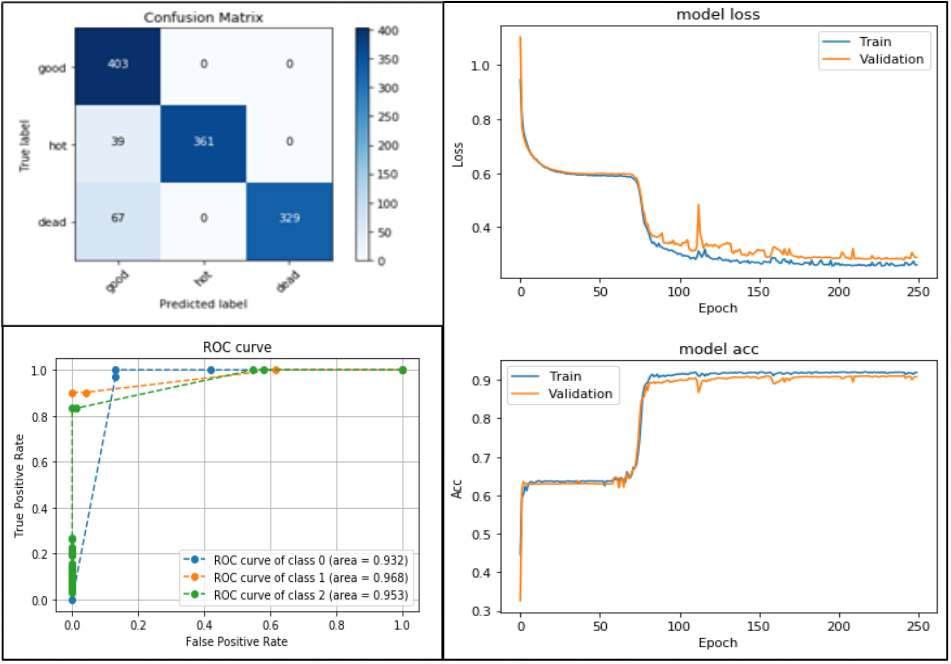
\includegraphics[width=\textwidth]{Performance_of_2nd_model.png}
\caption{Three convolutional layers model results\label{fig:model2results}}
\end{figure}

\subsection{Three Convolutional Layers with a new architecture for multiclass classification}

As can be seen in the CM of \autoref{fig:model2results}  that there is still scope to improve the prediction accuracy and minimize FPR.
  To achieve this, we introduce the use of BatchNorm before every activation layer as can be seen in the code snippet in \autoref{bestidmodel}.
  This model makes the CM more diagonal and brings the ROC AUC (Area Under the Curve) closer to 1 compared to previous model (previous section) as seen in \autoref{bestidmodelresults}.


\begin{figure}
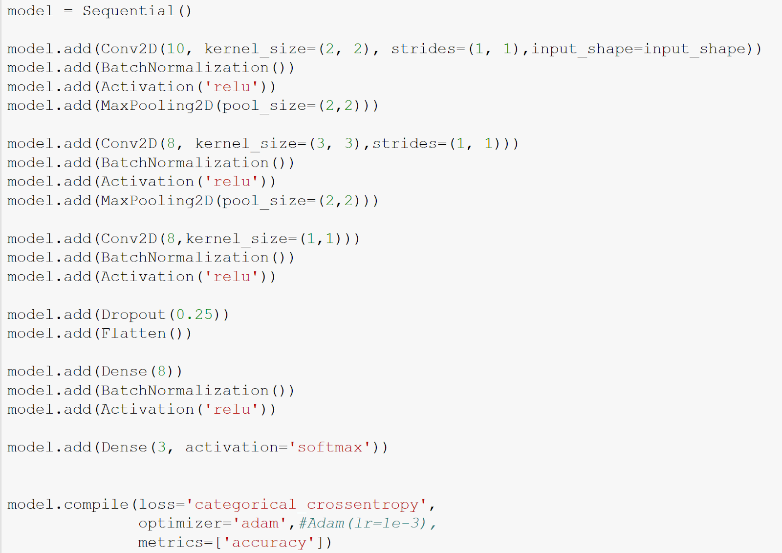
\includegraphics[width=\textwidth]{best_idmodel.png}
\caption{\label{bestidmodel}}
\end{figure}


\begin{figure}
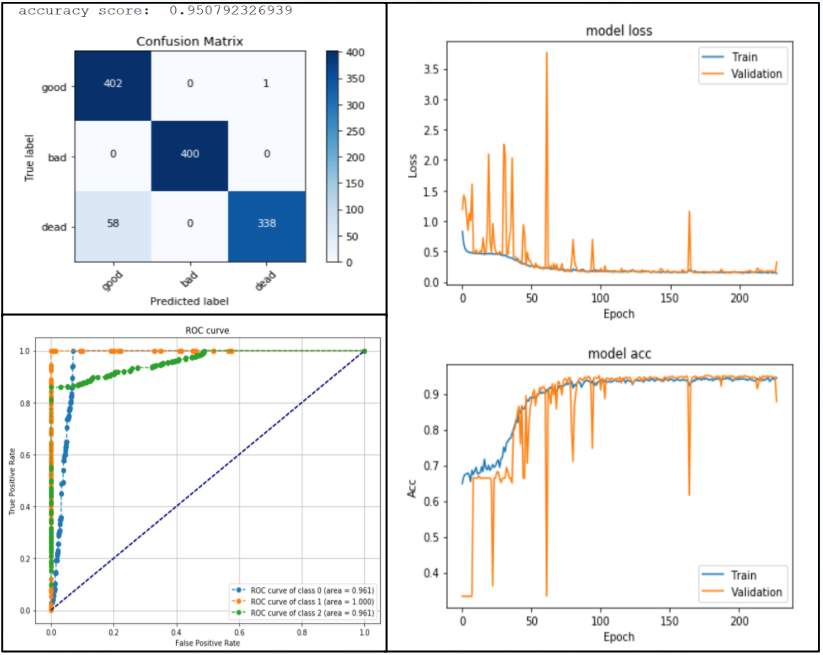
\includegraphics[width=\textwidth]{best_idmodelresults.png}
\caption{\label{bestidmodelresults}}
\end{figure}

\section{SSL Model for unknown anomalies in the HCAL data for DQM}

In this model, we try to generalize the learning strategy using SSL to identify unfamiliar anomalies in the HCAL DQM data. We use the reconstruction error as the discriminating factor to identify deviations from the good images. \autoref{fig:sslmodel} shows the code snippet for the SSL model.

\begin{figure}
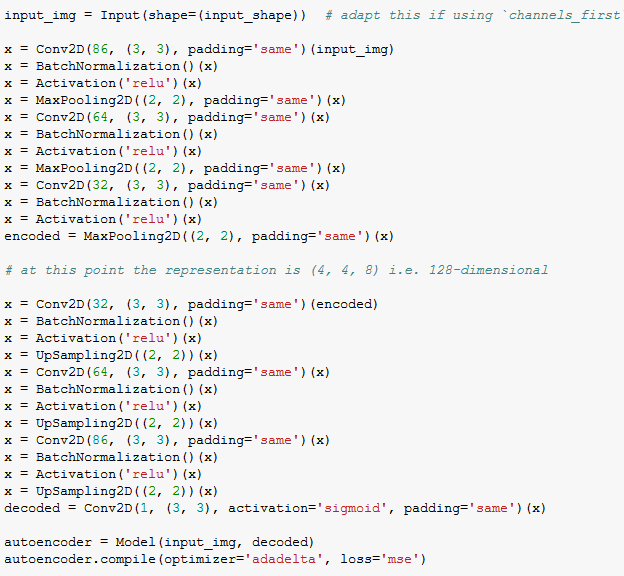
\includegraphics[width=\textwidth]{SSL_model.png}
\caption{\label{fig:sslmodel}}
\end{figure}

\autoref{SSLresults1} shows the input image, reconstruction image, and distance between the two for good, dead and hot scenarios with a $5\times5$ affected region. As can be seen from the maximum value of the vertical color bar for the distance map for each scenario, the good scenario has the least value; signifying efficient reconstruction and hence less error. 

\begin{figure}
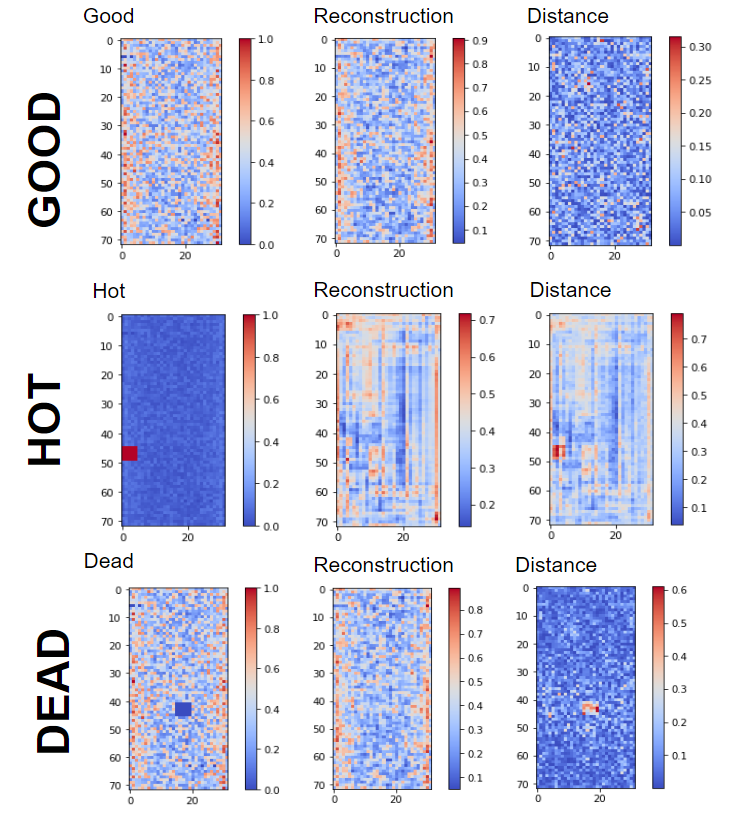
\includegraphics[width=\textwidth]{SSL_inputs_outputs.png}
\caption{Inputs, Reconstruction and distance maps for the SSL model\label{SSLresults1}}
\end{figure}

This also means that our model separates the three scenarios very well. This separation is highlighted in the histogram in \autoref{histo}. 


\begin{figure}
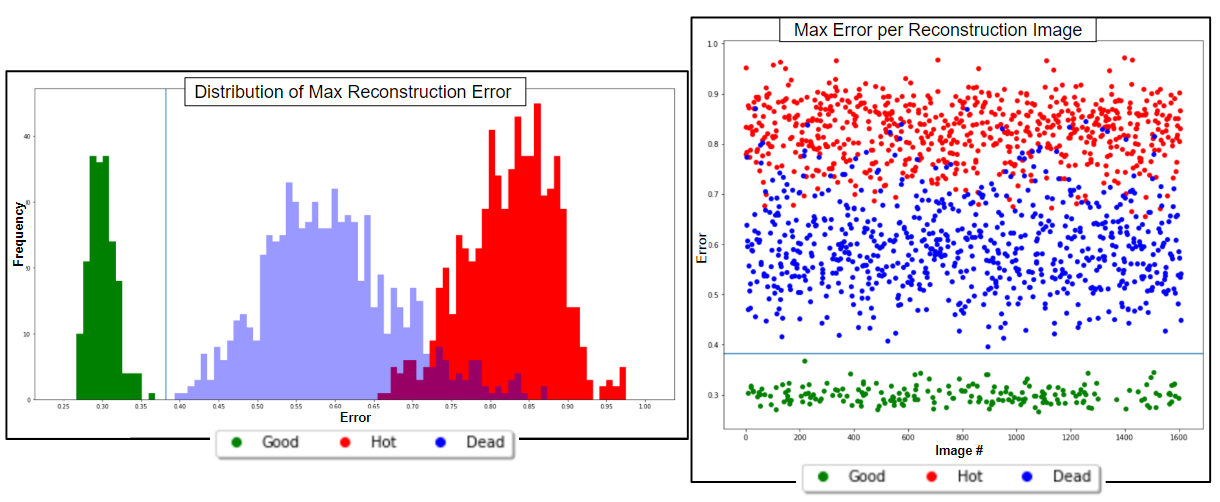
\includegraphics[width=\textwidth]{SSL_histo.png}
\caption{This histogram shows the distribution of error of the reconstruction and the dot plot on the right show the error of reconstruction of each image\label{histo}}
\end{figure}